%!TEX root = pixel-wise-street-segmentation.tex

\section{Related Work}\label{sec:related-work}
Road segmentation is a sub problem of general scene parsing or segmentation. In scene parsing every object in a scene is classified pixelwise with a label. Whereas in road segmentation often only two classes exist and more assumptions can be applied.\\
In the early days roads were usually annotated by color-based histogram approaches and specific model knowledge. Examples are the in 1994 introduced approach \cite{Beucher1990} using the watershed algorithm or \cite{aly2008real} where roads were annoted indirectly by lane markings found with a hough transformation.\\
Later insights of general scene parsing where transferred and more generic approaches like \cite{6182716} have achieved remarkable results with a Markov Random Field (MRF) and superpixels.\\
The impressive classification results of CNNs like AlexNet \cite{krizhevsky2012imagenet} or GoogleLeNet \cite{SzegedyLJSRAEVR14} during the the Google ImageNet LSVRC-2010 contest, made CNNs interesting for all kinds of computer vision problems like e.g. segmentation. \\
With \cite{long2014fully} Long and his team introduced a method for general scene parsing based on Fully Convolutional Networks (FCNs) and deconvolutional layer.\\
This approach is used as a blueprint to our implementation, described in Section \ref{sec:model}. Therefore the main concepts are introduced at the end of this section.\\
Instead of creating a new model, they converted existing classifaction CNNs like AlexNet or GoogleLeNet into FCNs. The obtained heatmaps for every class where calculated for multiple resolutions and upscaled with deconvolution layer interpolation to the original resolution.
With a fully connected convolutional layer in the end, the multiple outputs are combined into one classification heatmap for every class.\\

In \cite{mohan2014deep} a approach is presented, which makes also use of a CNNs in combination with deconvolution. In comparison to Long's network, among others it is less deep and uses less convolutional then deconvolutional layers. Furthermore the input image is divided in multiple patches and for each patch a separate neural network was trained. Their model achieved the best-recorded result on the same dataset we use, which is described in Section \ref{sec:datasets}.    

\subsection{CNN}
A CNN is bla.

\subsection{FCN}
Is CNN where bla.
\begin{figure}[htb]
	\centering
	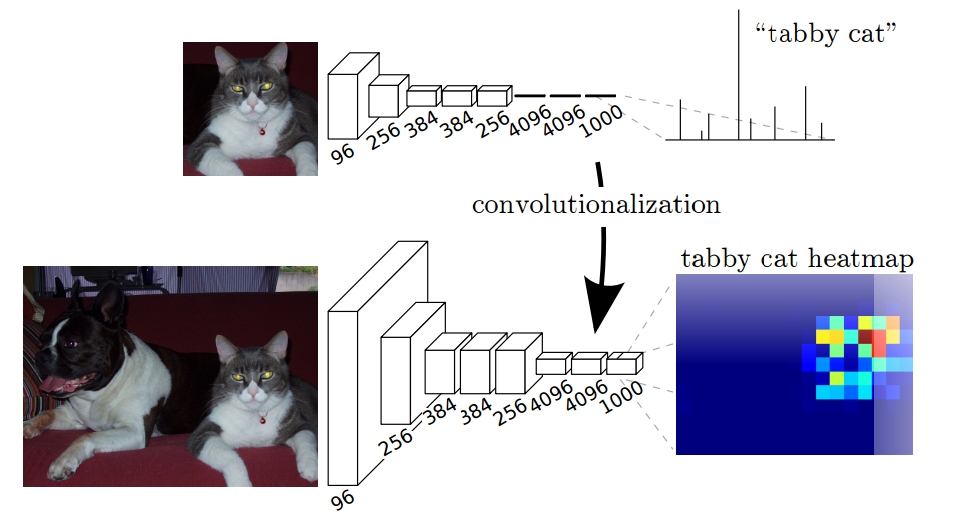
\includegraphics[width=9cm]{figures/fcnn}
	\caption{Comparison if a CNN for classifaction (top) and a FCN which creates a heatmap (bottom).}
\end{figure}

\subsection{Fully connected convolutional layer}
A fully connected convolutional layer is a regular convolutional layer in size of the input. Consequentially for every input pixel a weight is learned. Long noted in \cite{long2014fully} that it is the two dimensional equivalent to fully connected layer in a classification CNN.

\subsection{Deconvolutional Layer}
Deconv are mainly inversed convultions. Can be seen as inversed conv.
